
% .........................................
% Plantilla Latex en blanco
% .........................................




% -------------Estilo-------------

\documentclass[12pt,a4paper]{article}




% -------------Paquetes-----------

\usepackage[utf8]{inputenc} % Acentos
\usepackage[spanish]{babel} % Idioma (corte de palabras)
\usepackage{amsmath} % Matemáticas
\usepackage{amsfonts}
\usepackage{amssymb}
\usepackage{graphicx} % Gráficos




%------------Escritura en documento-----------


% Letras matemáticas de conjunto de números
% .........................................

\def\RR{\mathbb{R}}
\def\QQ{\mathbb{Q}}
\def\ZZ{\mathbb{Z}}
\def\NN{\mathbb{N}}




% Estilos de Teoremas
% ...................
 
\newtheorem{teor}{Teorema}[subsection]
\newtheorem{prop}{Proposición}[subsection]
\newtheorem{coro}{Corolario}[subsection]
\newtheorem{lema}{Lema}[subsection]
\newtheorem{defi}{Definición}[subsection]
\newtheorem{ejem}{Ejemplo}[subsection]
\newtheorem{ejer}{Ejercicio} [subsection]
\newtheorem{nota}{Nota}[subsection]




%-------------Portada------------

\title{Plantilla} 
\author{José Diamantino Hernández Guillén}
\date{\small{\today}}


\begin{document}

%---------Capítulo------
  
\include{chapter}

\section{Introducción}
\begin{defi}[Machine learning (aprendizaje automático)]
Diremos que se aplica machine learning cuando un programa aprende de la experiencia, respecto de una determinada tarea, a través del uso de una unidad de medida.
\end{defi}

Se pueden diferenciar dos tipos de machine learning:
\begin{enumerate}
\item Supervised learning (Apredizaje supervisado).
\item Unsupervised learning (Apredizaje no supervisado).
\end{enumerate}

\begin{defi}[Supervised learning]
Es un tipo de machine learning que da la respuesta correcta de una variable. 
\\\\
Ejemplo: Predicción del valor de una casa.
\end{defi}

\begin{defi}[Unsupervised learning]
Es un tipo de machine learning que proporciona las relaciones de nuestros datos. 
\\\\
Ejemplo: Búsqueda de noticias similares.
\end{defi}

A la hora de crear un algoritmo de machine learning es bueno considerar los siguientes consejos:
\begin{itemize}
\item Coleccionar muchos datos: la base de cualquier algoritmo son los datos. Cuantos más datos se tengan mejor.
\item Empezar con un algoritmo simple: Al principio es conveniente elegir las características más relevantes. Posteriormente en función de los resultados erróneos, se eligen características que puedan solventen dichos errores.
\item Hacer una lista de soluciones: Cuando un algoritmo no funciona es bueno realizar una lista de soluciones antes de tomar una decisión. Esto se debe a que algunas decisiones pueden llevar meses y no solventar el problema. Algunas soluciones que se consideran son: examinar más detenidamente los ejemplos que fallan, valorar si es mejor considerar más características o ejemplos, valorar la creación de datos artificiales (y el tiempo que supone)...
\end{itemize}


\subsection{Machine learning pipeline}
En ocasiones para obtener un resultado es necesario dividir el problema en varios sub-problemas de machine learning. Cada uno de estos sub-problemas serán tratados por separado en diferentes módulos. Para determinar en que módulo es necesario invertir más tiempo se utiliza el celling analisys. Este consiste en determinar el accuracy (exito) del modelo global según los diferentes módulos. Por ejemplo si tenemos cuatro módulos y obtenemos lo siguiente:

\begin{itemize}
\item Modelo global $\longrightarrow$ 72\% Accuracy
\item Modelo global con módulo 1 perfecto $\longrightarrow$ 73\% Accuracy
\item Modelo global con módulos 1 y 2 perfectos $\longrightarrow$ 84\% Accuracy
\item Modelo global con módulos 1, 2 y 3 perfectos $\longrightarrow$ 85\% Accuracy
\item Modelo global con módulos 1, 2, 3 y 4 perfectos $\longrightarrow$ 100\% Accuracy
\end{itemize}

Entonces los módulos más relevantes son el modulo 2 y el módulo cuatro, puesto que al estar perfectos (pasarles las respuestas correctas) obtenemos un aumento superior al 10\% en accuracy. Por lo tanto, sería necesario invertir más tiempo en estos.

\subsection{Elementos de machine learning}
Según el método que se utilice, se pueden observar los siguientes elementos:
\begin{itemize}
\item Sets (conjuntos)
\begin{enumerate}
\item Training Set (conjunto de entrenamiento-60\%): conjunto de datos que permiten que un modelo aprenda.
\item Cross Validation Set (conjunto de validación-20\%): conjunto de datos que permiten fijar los mejores parámetros del modelo.
\item Test Set (conjunto de prueba-20\%): conjunto de datos que determinan el error de un modelo.
\end{enumerate}
\begin{nota}[Mean normalization]
En muchas ocasiones en lugar de tomar directamente los conjuntos, se realiza una normalización de estos:
\begin{equation}
x_i \rightarrow \dfrac{x_i-\mu_i}{s_i}
\end{equation}
donde: 
\begin{itemize}
\item $\mu_i$: promedio de la variable $x_i$.
\item $s_i$: derivación estándar o $\max (x_i)$ - $\min (x_i)$
\end{itemize}
Generalmente se utiliza cuando para varios $i$ no se verifica:
$$x_i \in [-3,-1/3] \cup [1/3,3].$$
\end{nota}
\item Hypothesis (hipótesis)
\begin{itemize}
\item Función obtenida por el modelo para determinar la predicción de una solución al introducirle un ejemplo.
\end{itemize}
\item Cost function (función coste)
\begin{itemize}
\item Función que determina el error del modelo. En función del conjunto podemos distinguir tres tipos de errores:
\begin{itemize}
\item Training Cost Function: Determina el error del aprendizaje del modelo.
\item Cross Validation Cost Function: Determina el error del modelo según el parámetro que se utilice. 
\item Test Cost Function: Determina el error final del modelo (no depende de ningún parámetro).
\end{itemize}
\end{itemize}
\item Regularization (regularización)
\begin{itemize}
\item Control de las variaciones de los parámetros del modelo. 
\end{itemize}
\end{itemize}


\subsection{Machine Learning Diagnostic}
En función de los parámetros y datos del modelo podemos distinguir diferentes tipos de ajustes:

\begin{figure}[htb]
\center
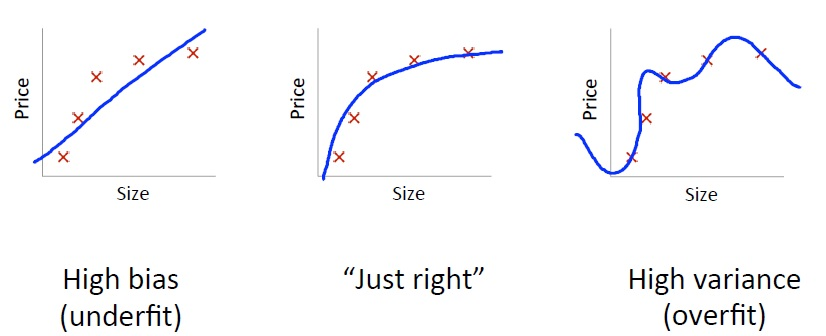
\includegraphics[width=0.7\textwidth]{diag}
\caption{Tipos de ajustes}
\end{figure}


En función de los parámetros que elijamos podemos obtener cada uno de los ajustes. El mejor ajuste es el ``just right'', el cual se corresponde con el menor cross-validation error. En función de cada parámetro (según este crezca o decrezca), se suele obtener la siguiente gráfica:

\begin{figure}[htb]
\center
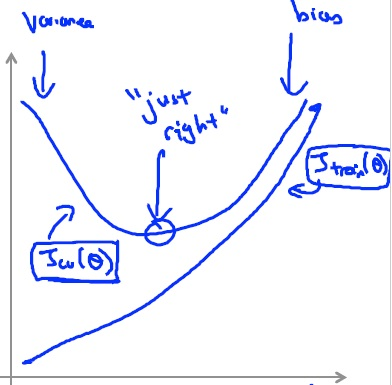
\includegraphics[width=0.4\textwidth]{error}
\caption{$J_{cv}$: Cross Validation Cost Function y $J_{train}$: Training Cost Function}
\end{figure}

De este modo se elegirán los parámetros del modelo para tener el mínimo cross-validation error. Además, para detectar si existe ``high variance'' o ``high bios'' se utilizan las curvas de apredizaje. Estas curvas tienen en cuenta las funciones $J_{cv}$ y $J_{train}$ en función del número de ejemplos:

\begin{figure}[htb]
\center
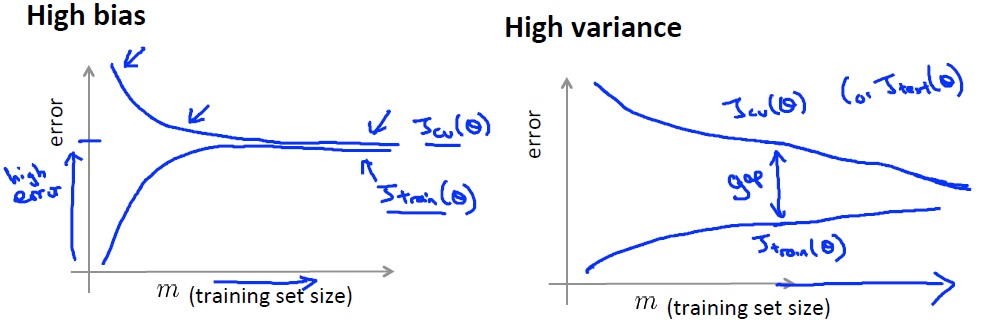
\includegraphics[width=0.9\textwidth]{learning_curve}
\caption{Curva de aprendizaje según el high bios y high variance}
\end{figure}

Cuando existe high bios las funciones convergen hacia un alto error. En cambio, cuando hay high variance existe un gran espacio entra las funciones. De este modo obtenemos dos opciones:
\begin{enumerate}
\item H.bios: El modelo no se ajusta a los datos. Es necesario usar una hipótesis más compleja: se añaden características, se añaden características polinómicas, se disminuye el parámetro de regularizazación...
\item H.variance: El modelo se sobre-ajusta a los datos. Es necesario usar una hipótesis más simple: se añaden más ejemplos, se quitan características, se aumenta el parámetro de regularizazación...
\end{enumerate}



\newpage

\section{Modelos}
En función del propósito podemos diferenciar varios modelos basados en machine learning:
\begin{itemize}
\item Value Prediction: Se utiliza para predecir valores de un ejemplo.

Modelos:
\begin{itemize}
\item \textbf{Linear/polynomial regression}.
\end{itemize}
Ejemplos: predecir el valor de una casa...
\item Clasification: Se utiliza para clasificar un ejemplo.

Modelos:
\begin{itemize}
\item \textbf{Logistic regression}: Para $n>>m$ ($n=10000$ y $m=10-1000$) o $n<<m$.
\item \textbf{Suport vector machine}: Para $n>>m$ ($n=10000$ y $m=10-1000$) -sin núcleo-. Para $n<m$ ($n=1-1000$ y $m=10000-50000$) -con núcleo-. Para $n<<m$ -sin núcleo-.
\item \textbf{Neural networks}: Obtiene de funciones complejas con menos coste computacional.
\end{itemize}
Ejemplos: email spam classification, predicción del tiempo, cancer classification...
\item Anomaly Detection: Se utiliza para detectar si un ejemplo es anómalo. A diferencia de los de clasificación, estos se utilizan cuando el número de ejemplos con $y=1$ es muy pequeño y $y=0$ es grande. También se usa cuando se esperan que las futuras anomalías no sean como las actuales.

Modelos:
\begin{itemize}
\item \textbf{Normal distribution}: Cuando m es pequeño o el coste computacional es alto.
\item \textbf{Multivariate gaussian distribution}: Cuando $m>n$ y el coste computacional es bajo.
\end{itemize}
Ejemplos: detección de usuarios distintos, fraude, monotorización de dispositivos...
\item Collaborative filtering: Se utiliza para obtener características de los ejemplos.

Modelos:
\begin{itemize}
\item \textbf{Collaborative filtering}: Se utiliza cuando tienes la opinión de varias personas sobre un mismo producto. Se pueden utilizar incluso si la mayoría de usuarios presentan pocas puntuaciones (la mayoría son 0).
\end{itemize}
Ejemplos: recomendar a usuarios películas en función de sus valoraciones, buscar libros (relacionados) que le guste a un usuario... 

\item Principal component analysis: Se utiliza para reducir el tamaño de los datos.

Modelos:
\begin{itemize}
\item \textbf{Principal component analysis}.
\end{itemize}
Ejemplos: reducir el coste computacional de un algoritmo, representar datos en 2D y 3D... No se utiliza para evitar el overfitting.

\item Online Learning: Se utiliza para tratar con datos que se reciben constantemente. Se adapta a la sociedad cambiante.

Modelos:
\begin{itemize}
\item \textbf{Online Learning}.
\end{itemize}
Ejemplos: Captación de tendencias de usuarios con las que realizar recomendaciones y ofertas especiales.
\end{itemize}

\newpage
\subsection{Linear/Polinomial regression}
\begin{figure}[htb]
\center
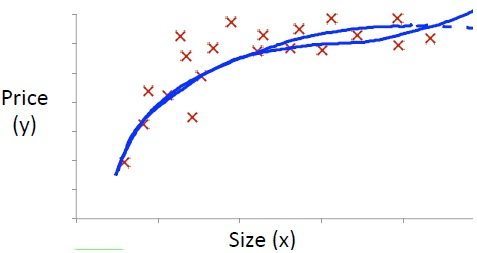
\includegraphics[width=0.5\textwidth]{linear_regresion}
\caption{Linear regression}
\end{figure}
\begin{itemize}
\item Hypothesis:
\begin{equation*}
h_\theta(x) = \theta_0 + \theta_1 x_1 + \theta_2 x_2 + ... + \theta_n x_n = \theta x 
\end{equation*}
donde $x_0=1$.
\begin{nota}
Para el caso polinómico realizamos lo siguiente: $x_1=x_1$, $x_2=x_1^2$, ..., $x_d=x_1^d$. De este modo obtenemos $h_\theta(x)=h_\theta(x_1)$.
\end{nota}
\item Cost Function:
\begin{equation*}
J(\theta)=\dfrac{1}{2 m} \sum_{i=1}^{m} (h_\theta(x^{(i)})-y^{(i)})+ \dfrac{\lambda}{2m} \sum_{i=1}^{n}\theta^{2}_j 
\end{equation*}
\item Parámetros desconocidos:
\begin{itemize}
\item $\theta \longrightarrow$ Training Set (Automático).
\item $\lambda \longrightarrow$ Cross Validation Set (Seleccionar).
\item $d  \longrightarrow$ Cross Validation Set (Manual).
\end{itemize}
\item Consejos:
\begin{itemize}
\item Hay que fijarse que la regularización no afecta al parámetro $\theta_0$.
\item La normalización de las variables es importante en el caso polinómico. 
\end{itemize}
\end{itemize}


\newpage
\subsection{Logistic regression}
\begin{figure}[htb]
\center
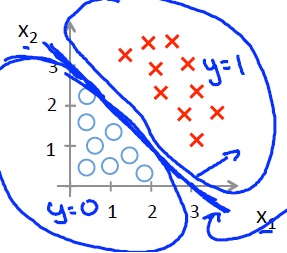
\includegraphics[width=0.4\textwidth]{logistic_regresion}
\caption{Logistic regression}
\end{figure}
\begin{itemize}
\item Hypothesis:
\begin{equation*}
h_\theta(x) = g(\theta x) 
\end{equation*}
donde $x_0=1$ y $g(z)=\dfrac{1}{1+e^{-z}}$ (sigmoid function).
\begin{nota}
Para el caso polinómico realizamos lo siguiente: $x_1=x_1$, $x_2=x_1^2$, ..., $x_d=x_1^d$. De este modo obtenemos $h_\theta(x)=h_\theta(x_1)$.
\end{nota}
\item Cost Function:
\begin{equation*}
J(\theta) = \dfrac{1}{m} \sum_{i=1}^{m} cost(h_{\theta}(x^{(i)}),y^{(i)}) + \dfrac{\lambda}{2 m} \sum_{j=1}^{n} \theta_{j}^{2} 
\end{equation*}
donde
\begin{equation*}
cost(h_{\theta}(x),y)=-y \log(h_{\theta}(x)) - (1-y) \log(1-h_{\theta}(x))  
\end{equation*}
\item Boundary
\begin{equation}
h_{\theta}(x) = P(y=1|x,\theta)
\end{equation}
Si consideremos que:
\begin{equation*}
h_{\theta}(x) \geq \alpha \Rightarrow y_{pred} = 1.
\end{equation*}
la frontera vendrá dada por:
\begin{equation*}
h_{\theta}(x) = \alpha.
\end{equation*}
Por lo tanto:
\begin{itemize}
\item Para predecir únicamente si se está seguro se aumenta el $\alpha$.
\item Para predecir si existe una mínima posibilidad se disminuye el $\alpha$.
\end{itemize}

\item Multi-class (one vs all)

\begin{figure}[htb]
\center
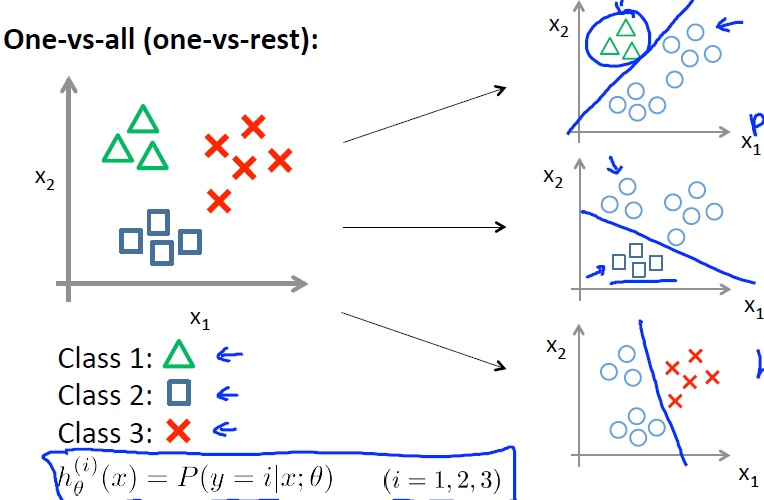
\includegraphics[width=0.6\textwidth]{one_all}
\caption{Logistic regression}
\end{figure}
Si y puede tener más de dos valores (1,2,3,4...) se utiliza multi-class clasification. Para ello se realizan tantas logistic regression como clases. Las logistic regression se realizan totalmente por separado considerando cada tipo como $y=1$ y el resto $y=0$. De este modo la hipótesis de predicción será:
\begin{equation*}
h_{\theta}(x) = \max_{i} h_{\theta}^{(i)}(x).
\end{equation*}
donde $h_{\theta}^{(i)}(x)$ son cada una de las hipótesis.
\item Parámetros desconocidos:
\begin{itemize}
\item $\theta \longrightarrow$ Training Set (Automático).
\item $\lambda \longrightarrow$ Cross Validation Set (Seleccionar).
\item $d  \longrightarrow$ Cross Validation Set (Manual).
\end{itemize}
\end{itemize}

\newpage

\subsection{Neural networks}
\begin{figure}[htb]
\center
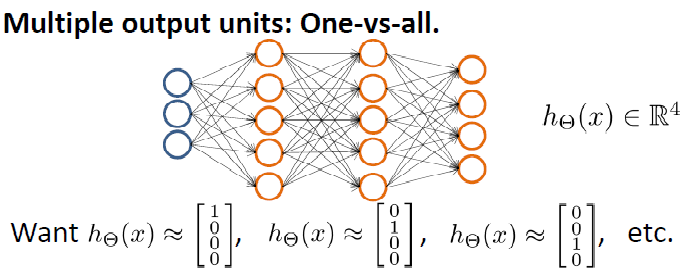
\includegraphics[width=0.9\textwidth]{neural_network}
\caption{Neural network}
\end{figure}
La layer 1 (capa 1) se denomina input layer. Por otro lado la capa final se denomina output layer. El resto de capas intermedias son las hidden layers.
\begin{itemize}
\item Hypothesis: 
\\

Forward propagation (ejemplo con 4 layers):
\begin{eqnarray*}
a^{(1)}&=&x\\
z^{(2)}&=&\theta^{(1)} a^{(1)}\\
a^{(2)}&=&g(z^{(2)})\\
z^{(3)}&=&\theta^{(3)} a^{(3)}\\
a^{(3)}&=&g(z^{(3)})\\
z^{(4)}&=&\theta^{(3)} a^{(3)}\\
h&=&g(z^{(4)})
\end{eqnarray*}
\item Cost Function:
\begin{equation*}
J(\theta)=-\dfrac{1}{m} \sum_{i=1}^{m} \sum_{k=1}^{K} (y_k^{(i)} \log(h_{\theta}^{k}(x^{i}))) + ((1-y_k^{(i)}) \log(1-h_{\theta}^{k}(x^{i}))) + \dfrac{\lambda}{2 m} \sum_{l=1}^{L-1} \sum_{i=1}^{S_{l}} \sum_{j=1}^{S_{l+1}} (\theta_{ji}^{(l)})^2
\end{equation*}

\item Parámetros desconocidos:
\begin{itemize}
\item $\theta \longrightarrow$ Training Set (Automático).
\item $\lambda \longrightarrow$ Cross Validation Set (Seleccionar).
\end{itemize}
\item Consejos:
\begin{itemize}
\item Para calcular las derivadas de la función coste se puede realizar Backpropagatión (mejora la velocidad para minimizar J).
\item Es necesario inicializar los parámetros de forma aleatoria: $\theta \in [-\epsilon,\epsilon]$.
\item Lo más usual es utilizar una capa oculta.
\item Cuantas más características tenga la capa oculta más compleja es la función hipótesis.
\item Si se utilizan varias capas ocultan, se suelen tomar del mismo tamaño. 
\end{itemize}
\end{itemize}

\newpage

\subsection{Suport Vector Machine}
\begin{figure}[htb]
\center
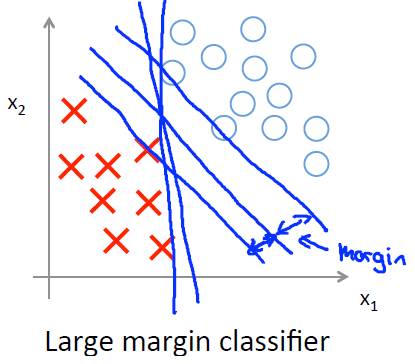
\includegraphics[width=0.5\textwidth]{suport_vector}
\caption{Suport Vector Machine}
\end{figure}
\begin{itemize}
\item Hypothesis: 
\[ h_{\theta}(x) = \left\{ \begin{array}{ll}
         1 & \mbox{si $\theta x \geq 0$};\\
         0 & \mbox{ en otro caso}.\end{array} \right. \]
\item Cost Function:
\begin{equation*}
J(\theta) = C \sum_{i=1}^{m} y^{(i)} cost_{1}(\theta x^{(i)})+(1-y^{(i)})cost_{0}(\theta x^{(i)})+\dfrac{1}{2} \sum_{j=1}^{n} \theta_{j}^2
\end{equation*}

\begin{figure}[htb]
\center
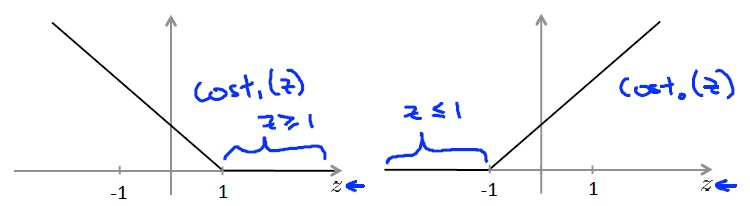
\includegraphics[width=0.8\textwidth]{suport_error}
\caption{Suport Vector Machine Cost}
\end{figure}

\item Núcleos:

\begin{itemize}
\item Se cambian las características para obtener decisiones no lineales.
\begin{equation*}
x_1, x_2, ..., x_n \longrightarrow f_1, f_2, ..., f_n
\end{equation*}
donde $f_i$ son los núcleos.
\item Gaussian Kernel:

\begin{figure}[htb]
\center
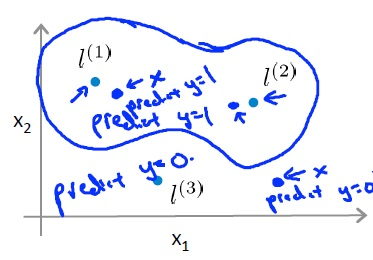
\includegraphics[width=0.5\textwidth]{suport_kernel}
\caption{Gaussian Kernels}
\end{figure}
\begin{equation*}
f_s = \exp(-\dfrac{||x-l^{(s)}||}{2 \sigma^{2}})
\end{equation*}
donde $l^{(s)}$ es un ejemplo. De este modo mide la distancia entre el punto $l^{(s)}$ y el ejemplo x, obteniéndose $m$ características.
\item Otros núcleos: Polynomial kernels: $k(x,l)= (x l + c_1)^{c_2}$, ... (satisfacen ``Mercer's Theorem'').
\end{itemize}

\item Parámetros desconocidos:
\begin{itemize}
\item $\theta \longrightarrow$ Training Set (Automático).
\item $C \longrightarrow$ Cross Validation Set (Seleccionar).
\item $\sigma \longrightarrow$ Cross Validation Set (Seleccionar).
\end{itemize}

\item Consejos:
\begin{itemize}
\item Utilizar librerías para implementarlo (falta por hacer).
\item Es importante normalizar las características antes de hacer los núcleos.
\item Los núcleos solo se aplican en Suport Vector Machine.
\end{itemize}
\end{itemize}


\newpage

\subsection{K-Means Algorithm}
\begin{figure}[htb]
\center
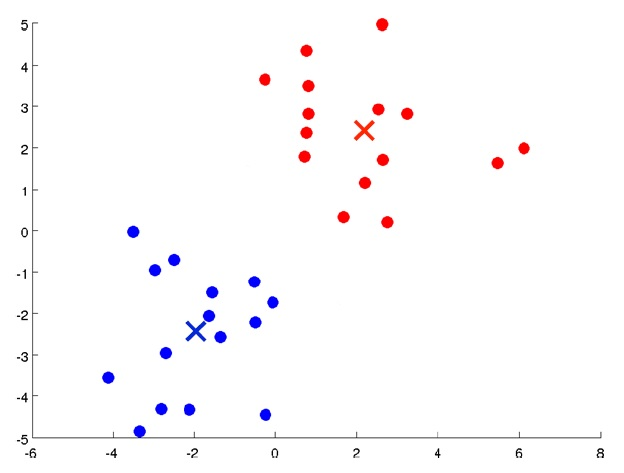
\includegraphics[width=0.4\textwidth]{k_means}
\caption{K-Means algorithm}
\end{figure}

\begin{itemize}
\item Process: 
\\
La función coste se minimiza en dos pasos:
\begin{enumerate}
\item Clasifica los puntos en función del centro que esté más cerca: $\min_{K} ||x^{(i)}-\mu_{k}||$
\item Una vez los puntos tienen asignado un centro, se mueve cada centro al punto promedio de los puntos con dicho centro asignado.
\begin{equation*}
\mu_k=\mbox{ promedio de los puntos asignados al claster K}
\end{equation*}
\end{enumerate}
\item Cost Function:
\begin{equation*}
J(\theta)=\dfrac{1}{m} \sum_{i=1}^{m} || x^{(i)}-\mu_{C^{(i)}}|| 
\end{equation*}
donde $C^{(i)}$ es el índice del centro $\mu_{C^{(i)}}$ al que $x^{(i)}$ ha sido asignado.
\item Parámetros desconocidos:
\begin{figure}[htb]
\center
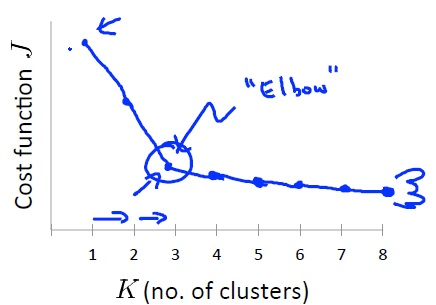
\includegraphics[width=0.4\textwidth]{elbow}
\caption{K-Means elbow}
\end{figure}
\begin{itemize}
\item $K$: El número de clasters se elige de dos modos:
\begin{itemize}
\item Método del codo: Se elige el número que se encuentre en el codo según el error para cada $K$ (no siempre existe).
\item En función del propósito: Por ejemplo en las ventas más clasters se corresponden con una mayor oferta pero más caro. Menos clasters se corresponden con una menor oferta pero más barato.
\end{itemize}
\end{itemize}
\item Consejos:
\begin{itemize}
\item La inicialización se realiza tomando como centros algunos puntos de $x^{(i)}$ de forma aleatoria.
\item Es bueno inicializar varias veces (puesto que en ocasiones falla) para que no coja soluciones no muy buenas, y coger la de menor coste.
\end{itemize}
\end{itemize}



\newpage

\subsection{Principal Component Analysis}
\begin{figure}[htb]
\center
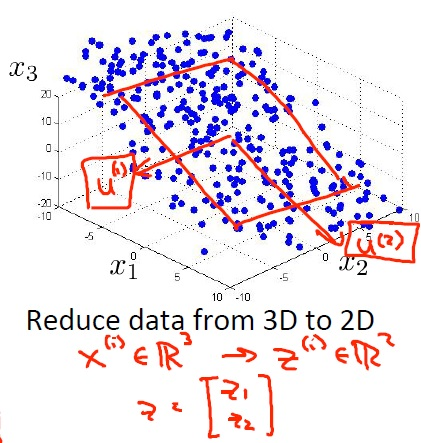
\includegraphics[width=0.4\textwidth]{pca}
\caption{PCA}
\end{figure}

\begin{itemize}
\item Calculo de vectores $U$:
\begin{equation*}
[U,S,V]=svd(Sigma) \mbox{ (también se puede utilizar $eig(Sigma)$)}.
\end{equation*}
\item Calculo de nuevos valores en dimensión reducida:
\begin{equation*}
Z=U_{reduce} X \mbox{ donde $U_{reduce}$ es $u_1, u_2, ..., u_r$}.
\end{equation*}
\item Cálculo de las proyecciones:
\begin{equation*}
x_{approx}=U_{reduce} Z
\end{equation*}
\item Parámetros desconocidos:
\begin{itemize}
\item $r$: El número de dimensiones finales. Se puede elegir de dos formas:
\begin{enumerate}
\item Se elige el primer $r$ que verifique:
\begin{equation*}
1-\dfrac{\sum_{i=1}^{r}S_{ii}}{\sum_{i=1}^{n}S_{ii}} \leq p
\end{equation*}
de modo que:
\begin{itemize}
\item Si $p=0.01$ $\Longrightarrow$ $99\%$ de varianza retenida.
\item Si $p=0.05$ $\Longrightarrow$ $95\%$ de varianza retenida.
\item Si $p=0.1$ $\Longrightarrow$ $90\%$ de varianza retenida.
\end{itemize}
\item Para representar los datos en 2D o 3D (r=2,3).
\end{enumerate}
\end{itemize}
\item Consejos:
\begin{itemize}
\item Es necesario normalizar los datos para hacer la reducción.
\item Si se aplica antes de realizar un algoritmo se aplica solo sobre el training set. Para los otros casos se utiliza $U_{reduce}$ (para trasformar los datos a menor dimensión).
\begin{itemize}
\item $x_1, x_2, ..., x_n \longrightarrow^{PCA} z_{1},z_2, ... ,z_{r}$ para Training Set.
\item $x_1, x_2, ..., x_n \longrightarrow^{U_{reduce}} z_{1},z_2, ... ,z_{r}$ para Cross and Test Sets.
\end{itemize}
\item Siempre es mejor probar primero sin PCA y posteriormente con PCA (se pierde cierta información al utilizar PCA).
\end{itemize}
\end{itemize}


\newpage

\subsection{Normal/Gaussian Distribution}

\begin{figure}[htb]
\center
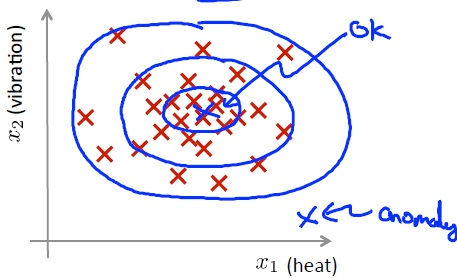
\includegraphics[width=0.4\textwidth]{norm_dist}
\caption{Normal/Gaussian Distribution}
\end{figure}

Caso - Normal distribution:
\begin{eqnarray*}
X &\sim& N(\mu,\sigma^{2})\\
\mu &=& \dfrac{1}{m} \sum_{i=1}^{m} x^{(i)}\\
\sigma^{2} &=& \dfrac{1}{m} \sum_{i=1}^{m} (x^{(i)}-\mu)^2 \equiv \dfrac{1}{m-1} \sum_{i=1}^{m} (x^{(i)}-\mu)^2 \\
p(x) &=& \prod_{j=1}^{n} \dfrac{1}{\sqrt{2 \pi} \sigma_{j}} \exp(- \dfrac{(x_j-\mu_j)^2}{2\sigma_j^{2}}) 
\end{eqnarray*}




\begin{itemize}
\item Detección de casos anómalos:
\begin{eqnarray*}
 p(X_t) & < & \epsilon \longmapsto \mbox{Caso anómalo}\\
 p(X_t) & \geq & \epsilon \longmapsto \mbox{Caso normal}
\end{eqnarray*}

\item Parámetros desconocidos:
\begin{itemize}
\item $\epsilon \longmapsto$  Cross validation set mediante el uso del F1 Score (si se tienen valores).
\end{itemize}
\item Consejos:
\begin{itemize}
\item Es importante la elección manual de características que obtenga relaciones de estas (Ej: $x_5=\dfrac{x_4^{2}}{x_{2}}$).
\item El algoritmo funciona incluso sin independencia de soluciones.
\item Es bueno tener o crear variables normales (sin normalizar). Para ello se pueden realizar transformaciones: $x_1 \longleftrightarrow \log(x_1+c), x_1 = x_1^{\frac{1}{3}}$...
\end{itemize}
\end{itemize}

Caso - Multivariate Normal distribution:
\begin{eqnarray*}
\mu &=& \dfrac{1}{m} \sum_{i=1}^{m} x^{(i)}\\
\sigma^{2} &=& \dfrac{1}{m} \sum_{i=1}^{m} (x^{(i)}-\mu)^2 \equiv \dfrac{1}{m-1} \sum_{i=1}^{m} (x^{(i)}-\mu)^2 \\
p(x) &=& \dfrac{1}{(2 \pi)^{n/2} |\sigma|^{1/2}} \exp(- \dfrac{1}{2} (X-\mu) \sigma^{-1} (X-\mu)) 
\end{eqnarray*}


\begin{itemize}
\item Detección de casos anómalos:
\begin{eqnarray*}
 p(X_t) & < & \epsilon \longmapsto \mbox{Caso anómalo}\\
 p(X_t) & \geq & \epsilon \longmapsto \mbox{Caso normal}
\end{eqnarray*}

\item Parámetros desconocidos:
\begin{itemize}
\item $\epsilon \longmapsto$  Cross validation set mediante el uso del F1 Score (si se tienen valores).
\end{itemize}
\item Consejos:
\begin{itemize}
\item Es bueno tener o crear variables normales (sin normalizar). Para ello se pueden realizar transformaciones: $x_1 \longleftrightarrow \log(x_1+c), x_1 = x_1^{\frac{1}{3}}$...
\end{itemize}
\item F1 Score:
\begin{eqnarray*}
P&=& \dfrac{True~positives}{True~positives+False~positives}     \mbox{ (Precision)}\\
R&=& \dfrac{True~positives}{True~positives+False~negatives}    \mbox{ (Recuperation)} \\
F1~Score &=& 2 \dfrac{P R}{P+R}
\end{eqnarray*}
\end{itemize}




\newpage

\subsection{Collaborative filtering}
\begin{figure}[htb]
\center
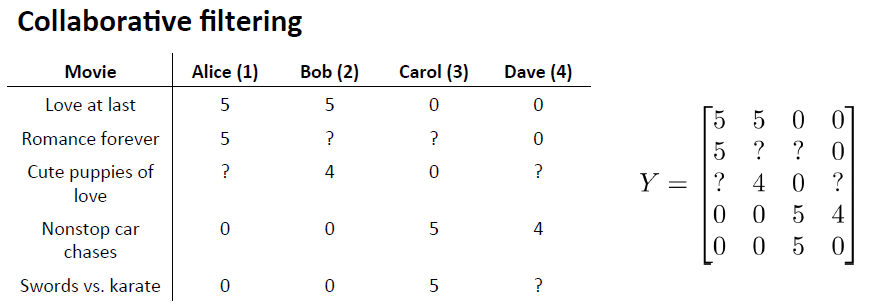
\includegraphics[width=0.8\textwidth]{cola_filt}
\caption{Collaborative filtering}
\end{figure}

\begin{itemize}
\item Hypothesis: 
\begin{equation*}
h_{\theta}(x)= \theta^{(j)} x^{(i)} \mbox{ opinión del usuario j para la ``pelicula'' i}
\end{equation*}
\item Cost Function:
\begin{equation*}
J(x,\theta) = \dfrac{1}{2} \sum_{(i,j):r(i,j)=1} (\theta^{(j)} x^{(i)}-y^{(i,j)})^2 + \sum_{i=1}^{n_m} \sum_{k=1}^{n} (x_{k}^{(i)})^2 + \dfrac{\lambda}{2} \sum_{j=1}^{n_m} \sum_{k=1}^{n} (\theta_k^{(j)})^2 
\end{equation*}

\item Parámetros desconocidos:
\begin{itemize}
\item $\theta, x \longrightarrow$ Training Set (Automático).
\item $\lambda \longrightarrow$ No se elige.
\end{itemize}
\item Consejos:
\begin{itemize}
\item Se inicializa $\theta$ y $x$ con valores aleatorios pequeños.
\item No existe $\theta_0$ ni $x_0$.
\item Es aconsejable realizar la normalización.
\item Si una película no tiene suficientes calificaciones, es mejor no incluirla.
\item Si se buscan encontrar películas relacionadas se utiliza: $|| x^{(i)} - x^{(j)} ||$.
\end{itemize}
\end{itemize}





\subsection{Online learning}
\begin{itemize}
\item $X$: Parámetros del usuario.
\item $\theta$: Parámetros del modelo.
\item $Y$: Acción del usuario.
\end{itemize}

\begin{itemize}
\item Process:
\begin{equation*}
(X,Y) \longmapsto \theta \mbox{ (se actualiza)} \longmapsto (X,Y) \mbox{ (se desecha y se toma el del siguiente)} 
\end{equation*}
\item Hypotesis y cost function:
\\
Logistic regression con un ejemplo.
\item Consejos:
\begin{itemize}
\item Las características a tener en cuenta se pueden obtener a partir de un sistema colaborativo.
\end{itemize}
\end{itemize}

\newpage

\section{Tratamiento de datos masivos}
Recolectar datos masivos ayuda si con estos un experto sería capaz de sacar el resultado, es decir, si las características están relacionadas con la predicción que se quiere hacer. En general, es mejor tener más datos, sin embargo, el coste computacional es mayor. 
\\

Una solución para tratar con datos masivos sería reducir las dimensiones de las características (PCA). Aún así, hay varios ejemplos que pueden suponer un problema. En los modelos, el principal problema del coste computacional se encuentra en la minimización de la función coste, para lo cual se suele utilizar el método del gradiente. Por ejemplo para el método linear regression el método del gradiente es: 

\begin{eqnarray*}
\theta_j &=& \theta_j - \alpha \dfrac{1}{m} \sum_{i=1}^{m} (h_{\theta}(x^{(i)})-y^{(i)})x_j^{(i)}   \\
j &=& 1,2,...,n.
\end{eqnarray*}

Alternativamente existen dos variantes con menor coste coputacional:

\begin{itemize}
\item Stochastic Gradient Descent
\begin{enumerate}
\item Ordenamiento aleatorio de los ejemplos.
\item 
\begin{eqnarray*}
\theta_j &=& \theta_j - \alpha (h_{\theta}(x^{(i)})-y^{(i)})x_j^{(i)}   \\
j &=& 1,2,...,n.
\end{eqnarray*}
\item Se hace para $i=1,...,m$.
\item Se repiten los dos pasos anteriores entre 1-10 veces.
\end{enumerate}
\item Mini-Batch Gradient Descent
\begin{enumerate}
\item Ordenamiento aleatorio de los ejemplos.
\item Se considera b=2-100 (usual b=10)
\item 
\begin{eqnarray*}
\theta_j &=& \theta_j - \alpha \dfrac{1}{b} \sum_{k=1}^{i+(b-1)} (h_{\theta}(x^{(k)})-y^{(k)})x_j^{(k)}   \\
j &=& 1,2,...,n.
\end{eqnarray*}
\item Se hace para $i=1,b+1,2b+1,...$.
\item Se repiten los dos pasos anteriores entre 1-10 veces.
\end{enumerate}
\end{itemize}

Además en los sumatorios de los métodos del "gradiente descenso" y "mini-batch gradient descent" se puede realizar un procesamiento en paralelo por núcleos o dispositivos (Multi-Core Machine). Al final una maquina junta los anteriores resultados de la computación en paralelo.

\subsection{Cost Function}
La función coste en el caso de stochastic gradient descent es:
\begin{equation*}
cost(\theta,(x^{(i)},y^{(i)})) = \dfrac{1}{2} (h(x^{(i)})-y^{(i)}) \mbox{ (se toma antes del ejemplo)}
\end{equation*}
Dibujando la función coste cada 1000 iteraciones (o más en caso de no observar una tendencia ascendente o descendente) obtenemos dos opciones:

\begin{figure}[htb]
\center
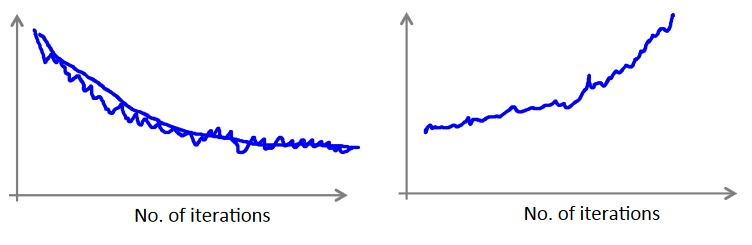
\includegraphics[width=0.8\textwidth]{cost_func}
\caption{Collaborative filtering}
\end{figure}

Si la tendencia es descendente el algoritmo funciona bien. En otro caso, es necesario elegir un $\alpha$ más pequeño. Las variantes no convergen con un $\alpha$ fijo sino que se quedan cerca del mínimo. Si se quiere que estos converjan se toma lo siguiente:

\begin{equation*}
\alpha \longmapsto \dfrac{\alpha}{cte_{iter}+cte_2}
\end{equation*}






\appendix
\section{Notación}

\begin{itemize}
\item $(X,Y)$: Training Set donde $X$ son las características e $Y$ son las respuestas correctas.
\item $J$: Cost Function.
\item $\theta$: Parámetros de aprendizaje.
\item $h_{\theta}(x)$: Hypothesis para el ejemplo $x=\{ x_1, x_2, ..., x_n\}$.
\item $x_i$: Característica $i$.
\item $x^{(i)}$: Ejemplo $i$.
\item $x_{j}^{(i)}$: Característica $j$ del ejemplo $i$.
\item $y^{(i)}$: Respuesta del ejemplo $i$.
\item $\lambda$: Parámetro de regularización.
\item $m$: Número de ejemplos del training set.
\item $n$: Número de características.
\end{itemize}




%---------Bibliografía-----

\addcontentsline{toc}{chapter}{Bibliography}
\renewcommand{\bibname}{Referencias}
\bibliography{refe}        
\bibliographystyle{plain}


\end{document}